\documentclass{article}

\usepackage[letterpaper,top=1.5cm,bottom=1.5cm,left=2cm,right=2cm,marginparwidth=1.75cm]{geometry}

\usepackage{graphicx}
\usepackage{booktabs}
\usepackage{float} 
\usepackage[colorlinks=true, allcolors=blue]{hyperref}
\usepackage[format=hang,font=small]{caption}
\usepackage{multirow} 

\title{Building a Model for A Biological Oscillator}
\author{Olivia Fernflores}
\date{November 10, 2024}

\begin{document}
\maketitle

\section{Introduction}

Biological oscillations, like the circadian rhythm, cell cycle, and segmentation clock, play an important role in dictating how biological systems function \cite{oscillationsimportance}. If we can model a biological oscillator, we can get a better understanding of how the system works under different conditions and how robust the system is to changes in parameter values. One model for a biological oscillator was presented in Elowitz and Leibler 2000, and they developed a synthetic network termed a represillator using transactional repressors that are not typically part of any biological clock in E.coli \cite{represillator}. In this paper, we explore the model of a represillator and try adding positive feedback loops to increase the model's robustness to changes in parameter values \cite{represillator}. 

\section{Model Development}

\subsection{Represillator}

The first model we explored for a biological oscillator is the represillator model presented in Elowitz and Leibler 2000 \cite{represillator}. This model has three nodes, \textit{A}, \textit{B}, and \textit{C}, which represent proteins. When \textit{A} is active, it represses \textit{B}. Active \textit{B} represses \textit{C}, and active \textit{C} represses \textit{A}. A schematic of this model can be seen in Figure 1.    

\begin{figure}[H]
    \centering
    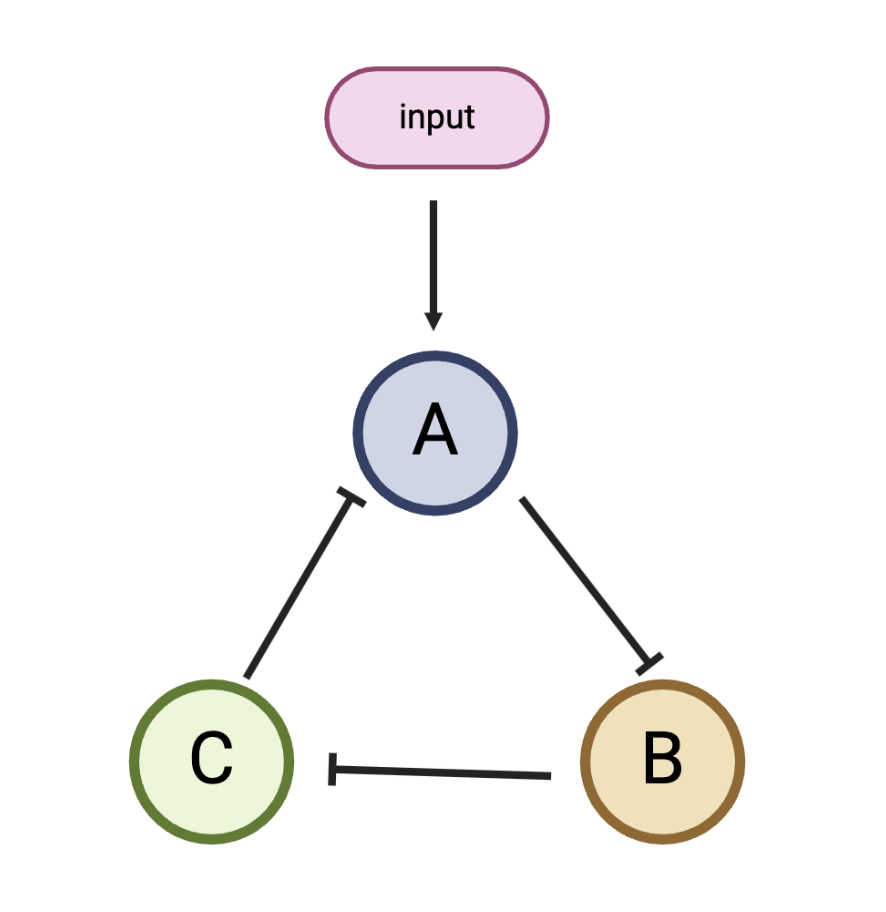
\includegraphics[width=0.4\textwidth]{figure1.png}
    \caption{Rpresillator built with proteins \textit{A}, \textit{B}, and \textit{C}. Each protein represses the protein at the next node and is repressed by the protein at the previous node. This is the model presented in Elowitz and Leibler 2000 \cite{represillator}.}
    \label{fig:1}
\end{figure}

The represillator can be represented by a set of three coupled differential equations to describe the change in concentration of active protein with respect to time. Using Michaelis-Menten kinetics, we can generally describe the activation and repression of a protein as follows:

\[
\text{Activation Rate} = k_{\text{activation}} \cdot \frac{(1 - X)}{(1 - X) + J_X}
\]

Where:
\begin{itemize}
    \item \( k_{\text{activation}} \) is the rate constant for the activation of protein \( X \).
    \item \( J_X \) is a parameter that modulates the strength of the activation.
    \item\( (1 - X) \) represents the fraction of the protein that is not yet fully activated, and \( (1 - X) + J_X \) ensures the saturation effect.
\end{itemize}

\[
\text{Repression Rate} = - k_{\text{repression}} \cdot \frac{X}{X + J_X^{n_X}}
\]

Where:
\begin{itemize}
    \item \( k_{\text{repression}} \) is the rate constant for the repression of protein \( X \) by the interacting protein.
    \item \( J_X \) is a parameter that controls the strength of the repression.
    \item \( n_X \) is the Hill coefficient, which determines the cooperativity of the repression. If \( n_X > 1 \), the repression becomes more sensitive and exhibits a steeper transition.
\end{itemize}

With these relationships in mind, we can put together our system of equations to represent the represillator network. 


\begin{enumerate}
    \item \(\frac{dA}{dt} &= I \cdot k_1 \cdot \frac{(1 - A)}{(1 - A) + J_1} - C \cdot k_4 \cdot \frac{A}{A + J_4^{n_1}}\)
    \\
    \\
    Where:
    \begin{itemize}
        \item \(I \cdot k_1 \cdot \frac{(1 - A)}{(1 - A) + J_1} \)represents the rate at which \textit{A} is activated at rate \textit{k1} with strength \textit{J1}. There is no Hill coefficient here because we assume activation to be non-cooperative. 
        \item \(C \cdot k_4 \cdot \frac{A}{A + J_4^{n_1}} \)represents the rate at which \textit{C} represses \textit{A} at rate \textit{k4}. The rate is multiplied by the fraction of \textit{A} that is repressed, \(\frac{A}{A + J_4^{n_1}}\), with the effect diminishing as the concentration of \textit{A} increases. 
    \end{itemize}
    \item \(\frac{dB}{dt} &= k_2 \cdot \frac{(1 - B)}{(1 - B) + J_2} - A \cdot k_5 \cdot \frac{B}{B + J_5^{n_2}}\)
    \\
    \\
    Where:
    \begin{itemize}
        \item \(k_2 \cdot \frac{(1 - B)}{(1 - B) + J_2} \)represents the rate at which \textit{B} is activated at rate \textit{k2} with strength \textit{J2}. There is no Hill coefficient here because we assume activation to be non-cooperative. 
        \item \(A \cdot k_5 \cdot \frac{B}{B + J_5^{n_2}} \)represents the rate at which \textit{A} represses \textit{B} at rate \textit{k5}. The rate is multiplied by the fraction of \textit{B} that is repressed, \(\frac{B}{B + J_5^{n_2}}\), with the effect diminishing as the concentration of \textit{B} increases. 
    \end{itemize}
    \item \(\frac{dC}{dt} &= k_3 \cdot \frac{(1 - C)}{(1 - C) + J_3} - B \cdot k_6 \cdot \frac{C}{C + J_6^{n_3}}\)
    \\
    \\
    Where:
    \begin{itemize}
        \item \(k_3 \cdot \frac{(1 - C)}{(1 - C) + J_3} \)represents the rate at which \textit{C} is activated at rate \textit{k3} with strength \textit{J3}. There is no Hill coefficient here because we assume activation to be non-cooperative. 
        \item \(B \cdot k_6 \cdot \frac{C}{C + J_6^{n_3}} \)represents the rate at which \textit{B} represses \textit{C} at rate \textit{k6}. The rate is multiplied by the fraction of \textit{C} that is repressed, \(\frac{C}{C + J_6^{n_3}}\), with the effect diminishing as the concentration of \textit{C} increases. 
    \end{itemize}
\end{enumerate}

The network modeled by these equations is able to oscillate under specific parameter conditions and concentrations of all three proteins continue to oscillate over time without diminishing periodicity and amplitude. However, the network is very sensitive to changes in specific parameter values and we sought to make the network more robust by sequentially adding positive feedback loops to one, two, and three nodes in the network. 

\subsection{Represillator + Positive Feedback at \textit{A}}

We hypothesized that adding positive feedback loops to the system would improve robustness to changes in parameter values and began by developing a model with a single positive feedback loop at node \textit{A} where \textit{A} activates itself as shown in Figure 2.

\begin{figure}[H]
    \centering
    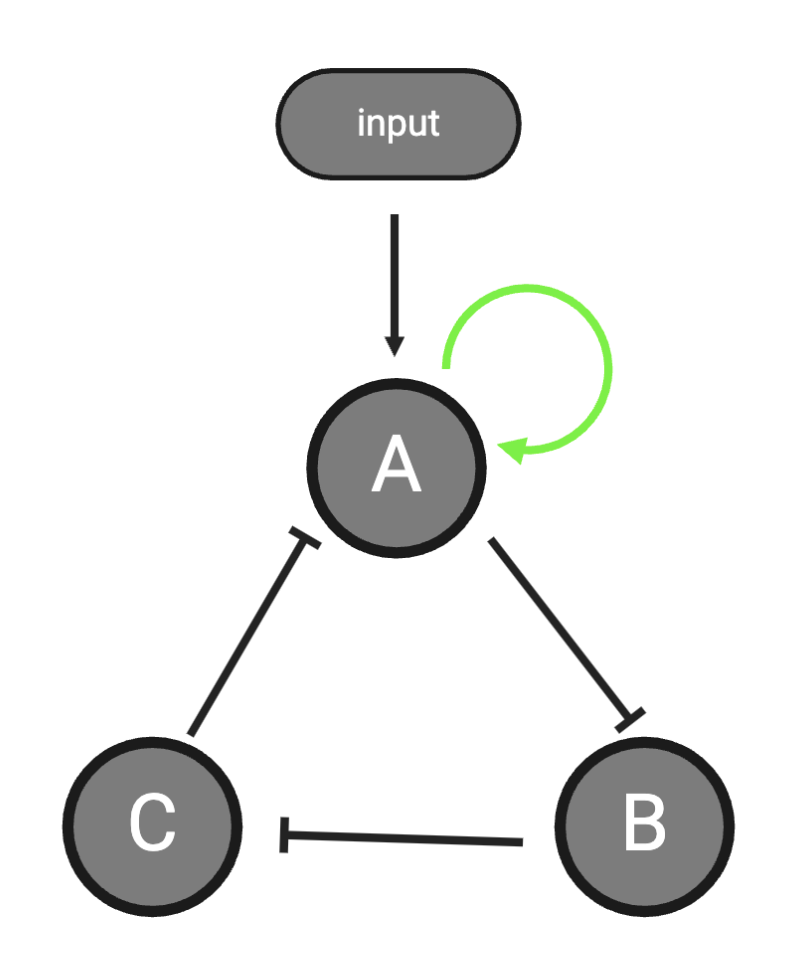
\includegraphics[width=0.4\textwidth]{figure2.png}
    \caption{Represillator + Positive Feedback at \textit{A}. The new relationship is shown in green and represents a positive feedback loop at \textit{A} where \textit{A} will activate itself.}
    \label{fig:2}
\end{figure}

To incorporate this additional positive feedback loop in our system of differential equations, we added an additional term to the equation for \( \frac{dA}{dt} that describes \textit{A} \)activating itself. 

\[
A \cdot k_a \cdot \frac{(1 - A)}{(1 - A) + J_a^{n_a}}
\]

The new term can be broken down as follows:
\begin{itemize}
    \item \( A \): The concentration of protein \textit{A}. As the concentration of \textit{A} increases, it drives its own production through positive feedback.
    \item \( k_a \): The rate constant for the positive feedback, which determines how strong the self-activation is.
    \item \( (1 - A) \): Represents the fraction of protein \textit{A} that is inactive (the maximum concentration of \textit{A} is 1).
    \item \( J_a \): Sets the threshold concentration at which the positive feedback becomes significant.
    \item \( n_a \): The Hill coefficient that controls the cooperativity of the feedback.
\end{itemize}

Adding this term to our equation for \(\frac{dA}{dt}\), we get the following set of equations for our system:

\begin{enumerate}
    \item \(\frac{dA}{dt} &= I \cdot k_1 \cdot \frac{(1 - A)}{(1 - A) + J_1} - C \cdot k_4 \cdot \frac{A}{A + J_4^{n_1}} + A \cdot k_a \cdot \frac{(1 - A)}{(1 - A) + J_a^{n_a}}\)
    \item \(\frac{dB}{dt} &= k_2 \cdot \frac{(1 - B)}{(1 - B) + J_2} - A \cdot k_5 \cdot \frac{B}{B + J_5^{n_2}}\)
    \item \(\frac{dC}{dt} &= k_3 \cdot \frac{(1 - C)}{(1 - C) + J_3} - B \cdot k_6 \cdot \frac{C}{C + J_6^{n_3}}\)
\end{enumerate}


\subsection{Represillator + Positive Feedback at \textit{A} + \textit{B}}

After adding one positive feedback loop, we were curious if adding a second positive feedback loop would make the system more robust. The single positive feedback loop at \textit{A} should improve robustness because it makes \textit{A} less dependent on \textit{B} and \textit{C}, so we wanted to see if reducing dependence in a similar way at \textit{B} would have a similar effect. As shown in Figure 3, we next incorporated a positive feedback loop at \textit{B}. 

\begin{figure}[H]
    \centering
    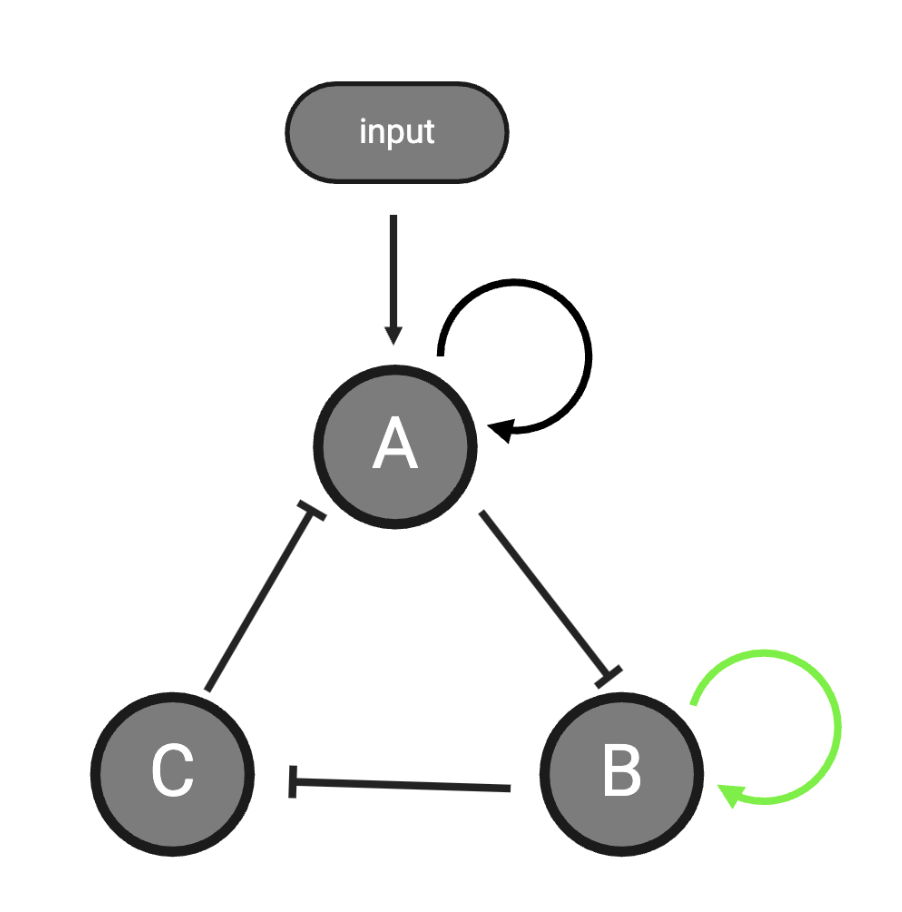
\includegraphics[width=0.4\textwidth]{figure3.png}
    \caption{Represillator + Positive Feedback at \textit{A} + \textit{B}. The new relationship is shown in green and represents a positive feedback loop at \textit{B} where \textit{B} will activate itself.}
    \label{fig:3}
\end{figure}

To update our system of equations accordingly, we must add a term to the equation for \(\frac{dB}{dt}\) that represents \textit{B} activating itself. This takes the same form as the term for \textit{A} activating itself. 

\[
B \cdot k_b \cdot \frac{(1 - B)}{(1 - B) + J_b^{n_b}}
\]

Again, the components of this term are:
\begin{itemize}
    \item \( B \): The concentration of protein \textit{B}. As the concentration of \textit{B} increases, it drives its own production through positive feedback.
    \item \( k_b \): The rate constant for the positive feedback, which determines how strong the self-activation is.
    \item \( (1 - B) \): Represents the fraction of protein \textit{B} that is inactive (the maximum concentration of \textit{B} is 1).
    \item \( J_b \): Sets the threshold concentration at which the positive feedback becomes significant.
    \item \( n_b \)*: The Hill coefficient that controls the cooperativity of the feedback.
\end{itemize}

Adding this term to our equation for \(\frac{dB}{dt}\), we get the following set of equations for our system:

\begin{enumerate}
    \item \(\frac{dA}{dt} &= I \cdot k_1 \cdot \frac{(1 - A)}{(1 - A) + J_1} - C \cdot k_4 \cdot \frac{A}{A + J_4^{n_1}} + A \cdot k_a \cdot \frac{(1 - A)}{(1 - A) + J_a^{n_a}}\)
    \item \(\frac{dB}{dt} &= k_2 \cdot \frac{(1 - B)}{(1 - B) + J_2} - A \cdot k_5 \cdot \frac{B}{B + J_5^{n_2}} + B \cdot k_b \cdot \frac{(1 - B)}{(1 - B) + J_b^{n_b}}\)
    \item \(\frac{dC}{dt} &= k_3 \cdot \frac{(1 - C)}{(1 - C) + J_3} - B \cdot k_6 \cdot \frac{C}{C + J_6^{n_3}}\)
\end{enumerate}

\subsection{Represillator + Positive Feedback at \textit{A} + \textit{B} + \textit{C}}

Finally, we considered adding positive feedback to all three nodes in the system. We hypothesized that having all three nodes controlled by positive feedback would make the system significantly more robust to changes in parameter values because it would make each node less dependent on the activity of other nodes. 

\begin{figure}[H]
    \centering
    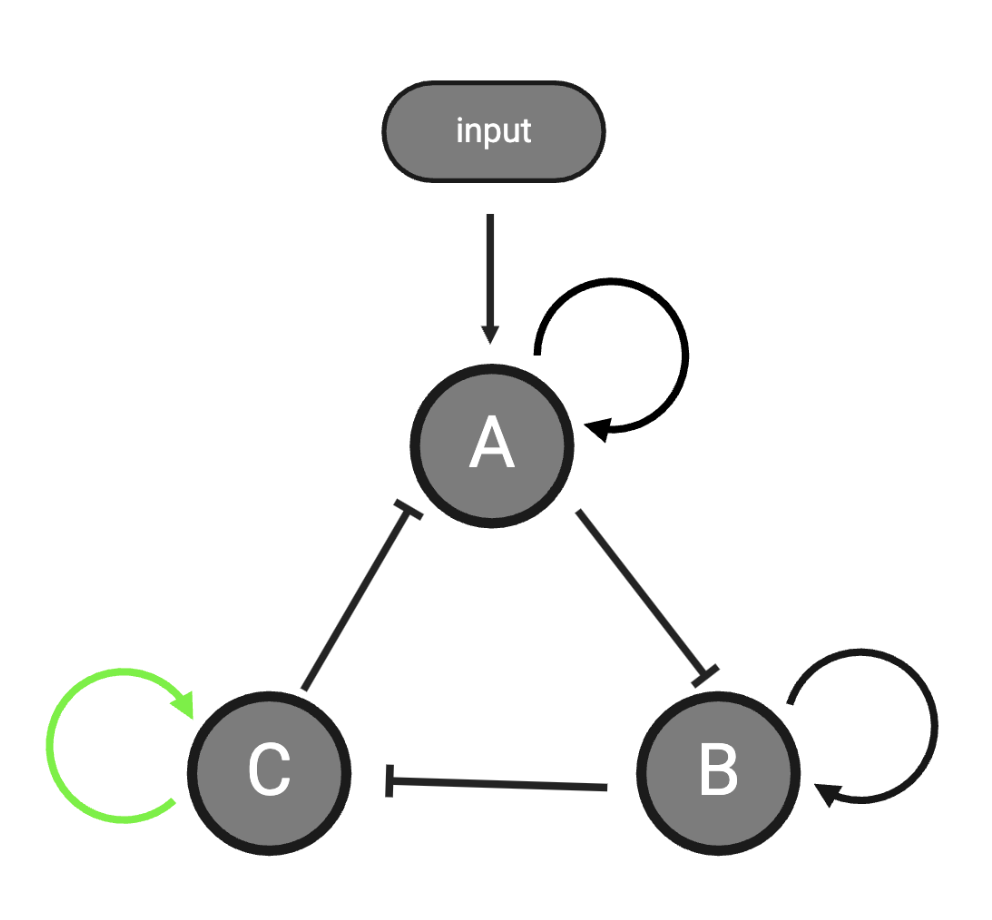
\includegraphics[width=0.4\textwidth]{figure4.png}
    \caption{Represillator + Positive Feedback at \textit{A} + \textit{B} + \textit{C}. The new relationship is shown in green and represents a positive feedback loop at \textit{C} where \textit{C} will activate itself.}
    \label{fig:4}
\end{figure}

Just as in the previous two sections, we needed to add a term to our equation for \(\frac{dC}{dt}\) to describe \textit{C} activating itself. This will be the same type of term we have added to our equations for \(\frac{dA}{dt}\) and \(\frac{dB}{dt}\).

\[
C \cdot k_c \cdot \frac{(1 - C)}{(1 - C) + J_c^{n_c}}
\]

With the new term added, the following set of equations models our system:

\begin{enumerate}
    \item \(\frac{dA}{dt} &= I \cdot k_1 \cdot \frac{(1 - A)}{(1 - A) + J_1} - C \cdot k_4 \cdot \frac{A}{A + J_4^{n_1}} + A \cdot k_a \cdot \frac{(1 - A)}{(1 - A) + J_a^{n_a}}\)
    \item \(\frac{dB}{dt} &= k_2 \cdot \frac{(1 - B)}{(1 - B) + J_2} - A \cdot k_5 \cdot \frac{B}{B + J_5^{n_2}} + B \cdot k_b \cdot \frac{(1 - B)}{(1 - B) + J_b^{n_b}}\)
    \item \(\frac{dC}{dt} &= k_3 \cdot \frac{(1 - C)}{(1 - C) + J_3} - B \cdot k_6 \cdot \frac{C}{C + J_6^{n_3}} + C \cdot k_c \cdot \frac{(1 - C)}{(1 - C) + J_c^{n_c}}\)
\end{enumerate}


\section{Results}

\subsection{Finding Parameter Values for the Represillator that allow Oscillation}

The first step in this project was to find a set of parameter values that allow the represillator to oscillate. Using the guidelines in Elowitz and Leibler 2000 \cite{represillator}, we did a parameter sweep across \textit{J} values from \( 10^{-2} \) to \( 10^{2} \), \textit{k} values from \( 10^{-2} \) to \( 10^{2} \), and \textit{n} values of 1 and 2 using initial concentrations of 0.5, 0.5, and 0.5 for \textit{A}, \textit{B}, and \textit{C} respectively and an input strength of 1.  We then examined the behavior of the system as we varied each of 15 parameters in our differential equations while keeping the rest constant. These results are summarized below in Figure 5 and Table 1.  

%oscillatory_behavior_baseline.pdf, oscillator_behavior_baseline_log.pdf

\begin{figure}[H]
    \centering
    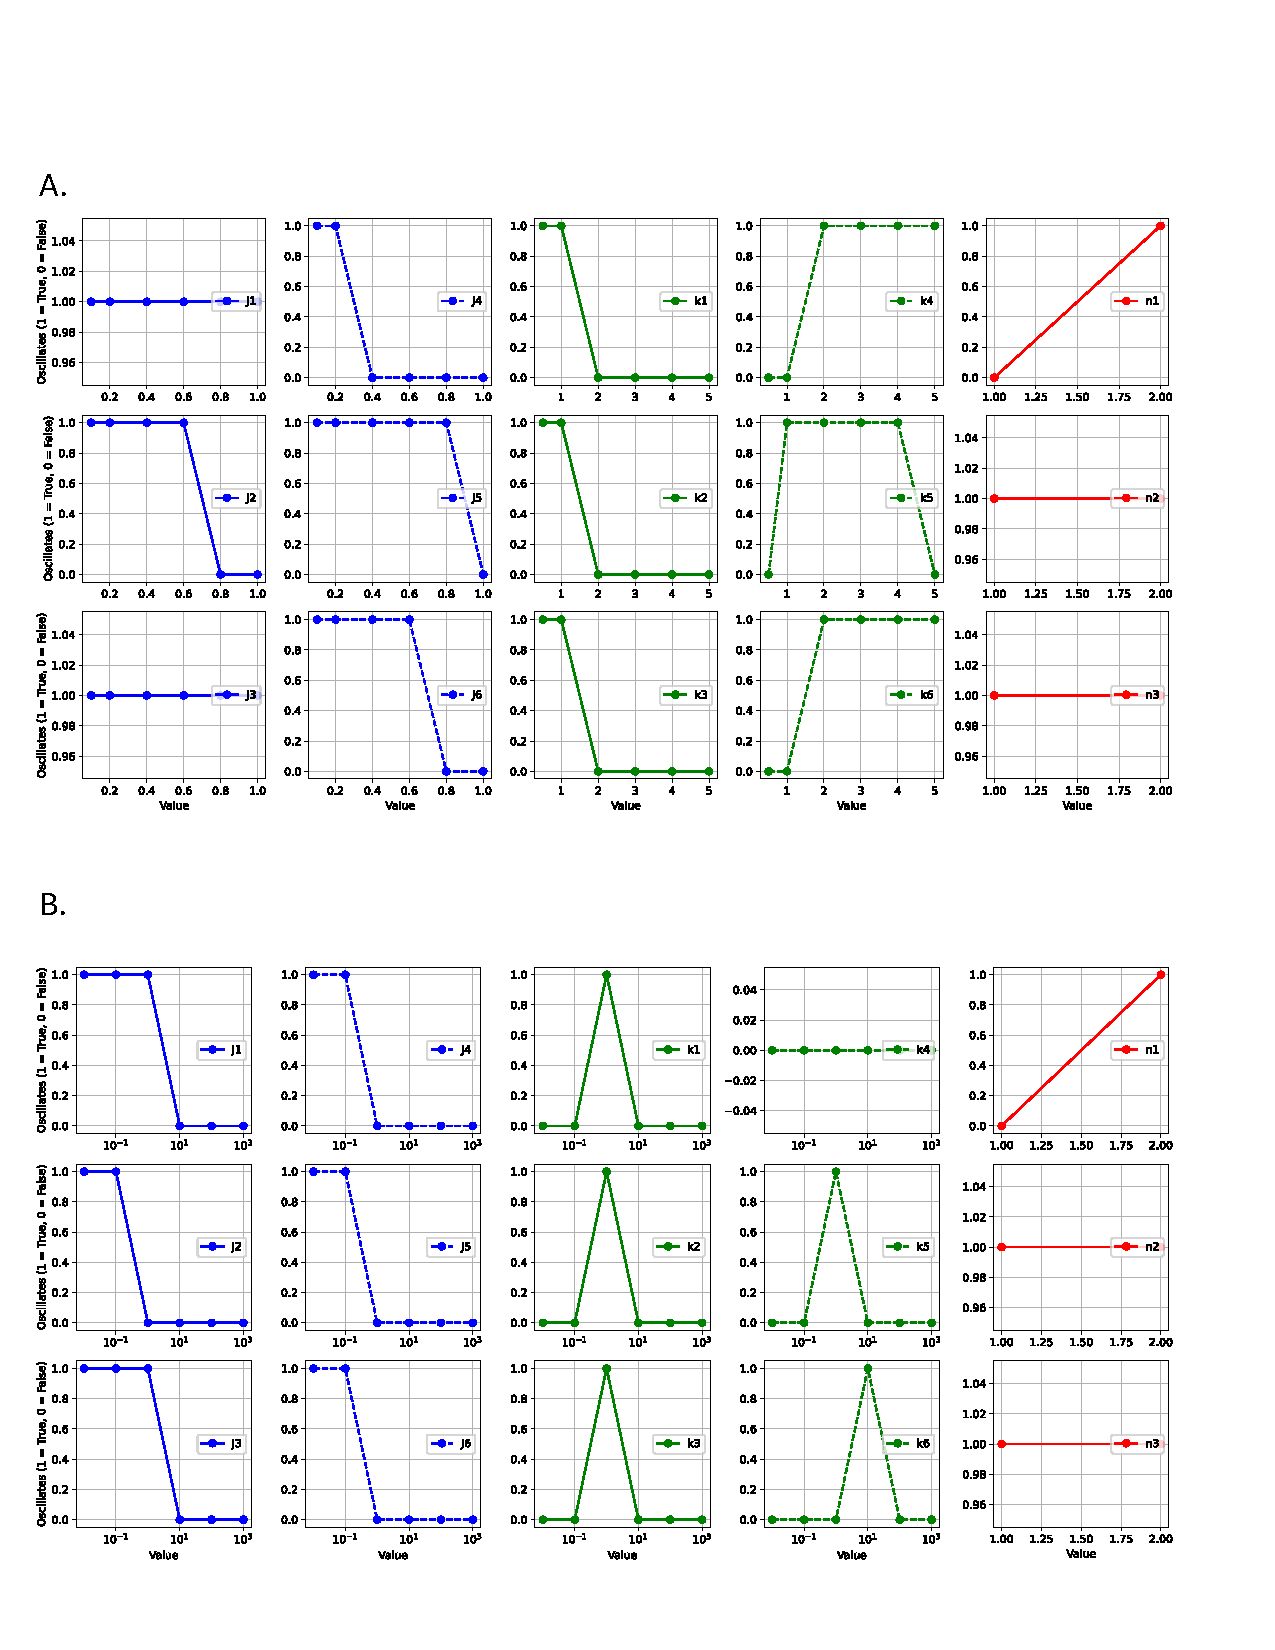
\includegraphics[width=0.7\textwidth]{figure5.pdf}
    \caption{Parameter sweep results for a basic represillator model. When the y-value is 1, the concentrations of all three proteins oscillate. When the y-value is 0, the concentration of at least one protein does not oscillate. A. The results of a parameter sweep done using \textit{J} values from 0.1 to 1 and \textit{k} values from 1 to 5. B. The results of a parameter sweep done using \textit{J} values from \( 10^{-2} \) to \( 10^{2} \), \textit{k} values from \( 10^{-2} \) to \( 10^{2} \)}. 
    \label{fig:5}
\end{figure}


\begin{table}[H]
\centering
\begin{tabular}{|l|l|l|}
\hline
\textbf{Parameter} & \textbf{Small Scale} &  \textbf{Log Scale} \\
\hline
J1 & 0.1, 0.2, 0.4, 0.6, 0.8, 1 & 0.01, 0.1, 1\\
J2 & 0.1, 0.2, 0.4, 0.6 & 0.01, 0.1\\
J3 & 0.1, 0.2, 0.4, 0.6, 0.8, 1 & 0.01, 0.1, 1\\
J4 & 0.1, 0.2 & 0.01, 0.1\\
J5 & 0.1, 0.2, 0.4, 0.6, 0.8 & 0.01, 0.1\\
J6 & 0.1, 0.2, 0.4, 0.6 & 0.01, 0.1\\
k1 & 0.5, 1 & 1\\
k2 & 0.5, 1 & 1\\
k3 & 0.5, 1 & 1\\
k4 & 2, 3, 4, 5 & None\\
k5 & 1, 2, 3, 4 & 10\\
k6 & 2, 3, 4, 5 & 10\\
n1 & 2 & 2\\
n2 & 1, 2 & 1, 2\\
n3 & 1, 2 & 1, 2\\
\hline
\end{tabular}
\caption{Parameter Values Explored in Parameter Sweep of Represillator model.}
\end{table}

One set of parameters from this sweep was selected (Table 2) and the behavior of the system under those parameters is shown in Figure 6. These parameter values will be held constant for the rest of the paper unless specified otherwise and will be called "oscillatory parameters". 

\begin{table}[H]
\centering
\begin{tabular}{|l|l|}
\hline
\textbf{Parameter} & \textbf{Value} \\
\hline
k1 & 1 \\
k2 & 0.5 \\
k3 & 1 \\
k4 & 2 \\
k5 & 2 \\
k6 & 2 \\
J1 & 0.2 \\
J2 & 0.2 \\
J3 & 0.3 \\
J4 & 0.2 \\
J5 & 0.2 \\
J6 & 0.3 \\
n1 & 2 \\
n2 & 2 \\
n3 & 2 \\
\hline
\end{tabular}
\caption{Oscillatory Parameters}
\end{table}


%concentration_over_time_baseline.pdf
\begin{figure}[H]
    \centering
    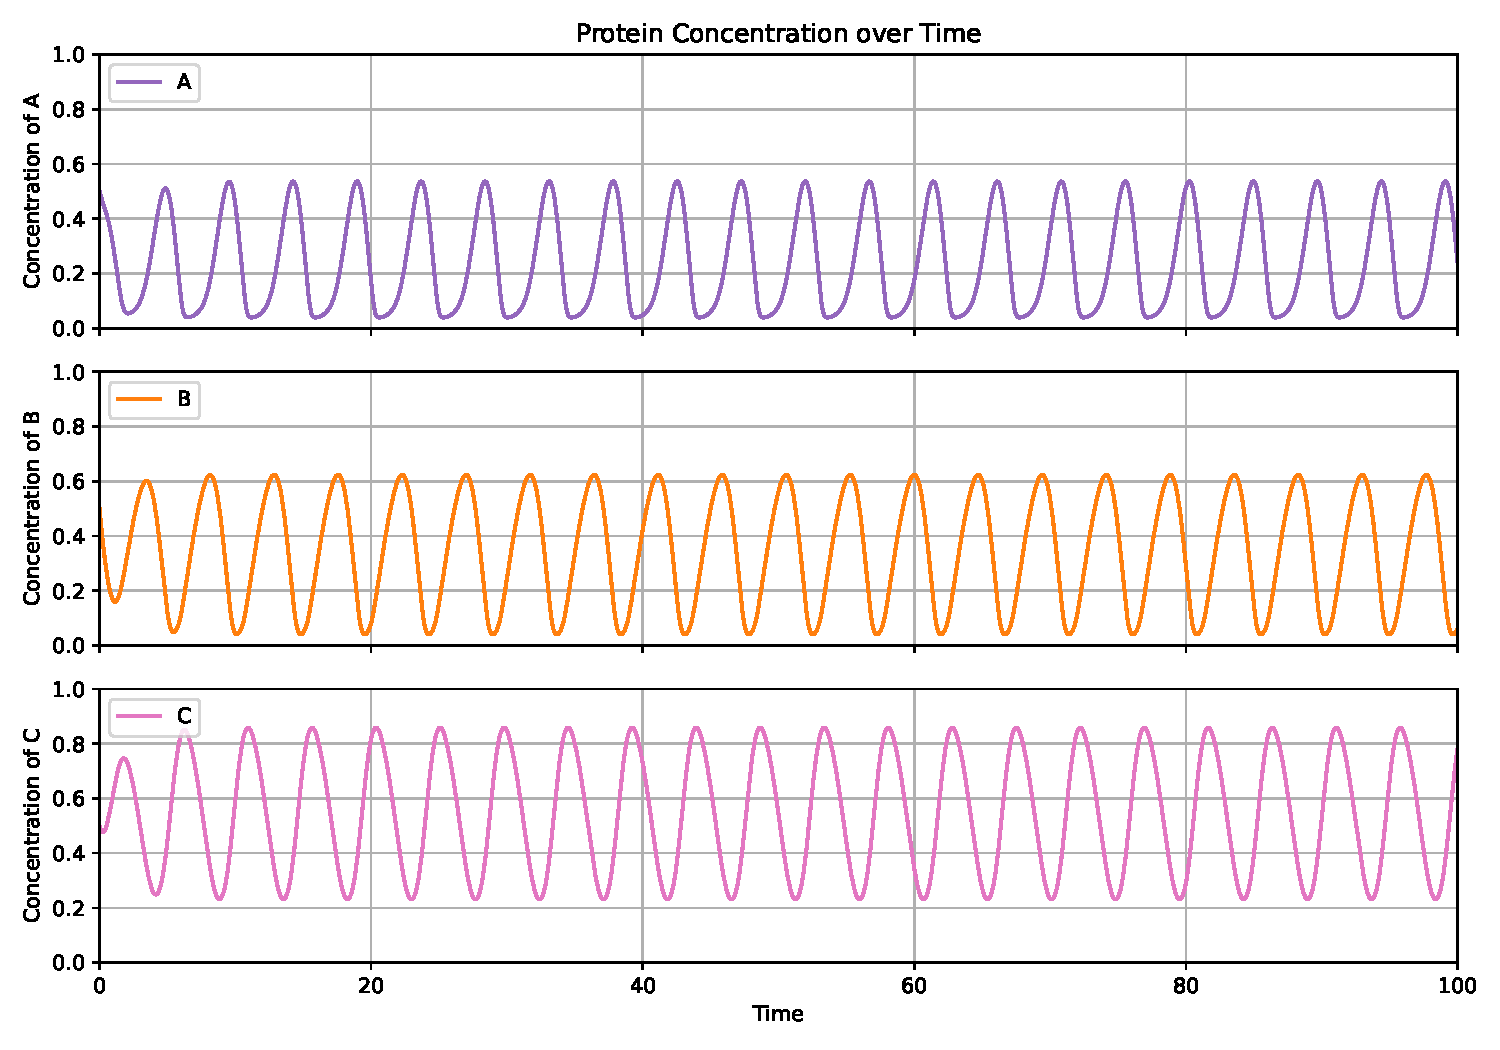
\includegraphics[width=0.7\textwidth]{/Users/olivia/Documents/Fall 2024/MCB 580/MCB580_Challenge3/plots/concentration_over_time_baseline.pdf}
    \caption{The behavior of the Represillator model under our oscillatory parameters.}
    \label{fig:6}
\end{figure}

This circuit clearly oscillates for all three proteins, but it is not very robust to changes in parameter values. Using the three models presented above with additional feedback loops, we held our oscillatory parameters constant and modeled each of our more complex systems, then tested each system for robustness to changes in parameter values. 


\subsection{Represillator + Positive Feedback at \textit{A}}

Using our oscillatory parameters from the previous section and the set of equations previously presented for our new model, we found that the system of a represillator with a positive feedback loop at \textit{A} does oscillate under the oscillatory parameters for all three proteins as shown in Figure 7. 

%concentration_over_time_A_positive_new_equations.pdf 
\begin{figure}[H]
    \centering
    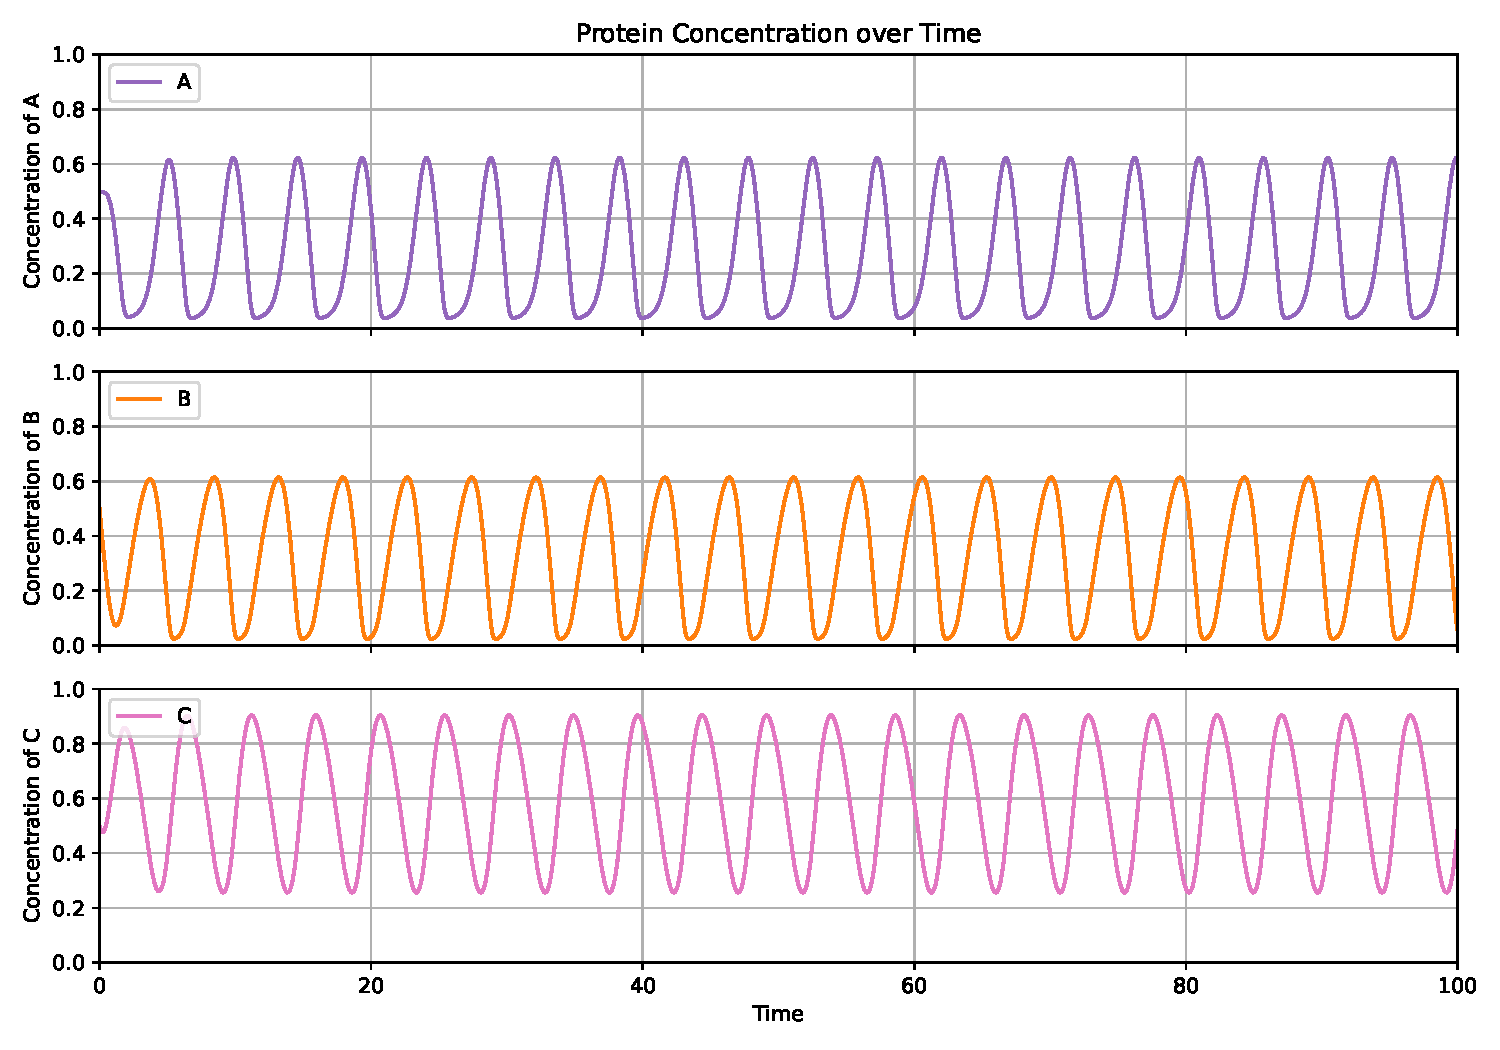
\includegraphics[width=0.7\textwidth]{/Users/olivia/Documents/Fall 2024/MCB 580/MCB580_Challenge3/plots/concentration_over_time_A_positive_new_equations.pdf}
    \caption{The behavior of the Represillator + Positive Feedback at \textit{A} model under oscillatory parameters.}
    \label{fig:7}
\end{figure}



Once we saw that this model was also oscillatory under our parameter set, we tested the robustness of this model compared to the represillator network. Again, using our oscillatory parameters set, we perturbed individual parameters holding the rest constant and examined the range under which the circuit still displayed oscillatory behavior. Although adding positive feedback at node \textit{A} was not enough to show robustness to parameter changes across all parameters used in the simple represillator model, we did see improved robustness in response to changes in specific parameters. In Figure 8, the results of our parameter sweep are shown, using the same parameter sweep ranges as the previous section (\textit{J} values from \( 10^{-2} \) to \( 10^{2} \), \textit{k} values from \( 10^{-2} \) to \( 10^{2} \)}, and \textit{n} values of 1 and 2). 

%oscillatory_behavior_A_positive_log_new_equations.pdf, oscillatory_behavior_A_positive_new_equations.pdf

\begin{figure}[H]
    \centering
    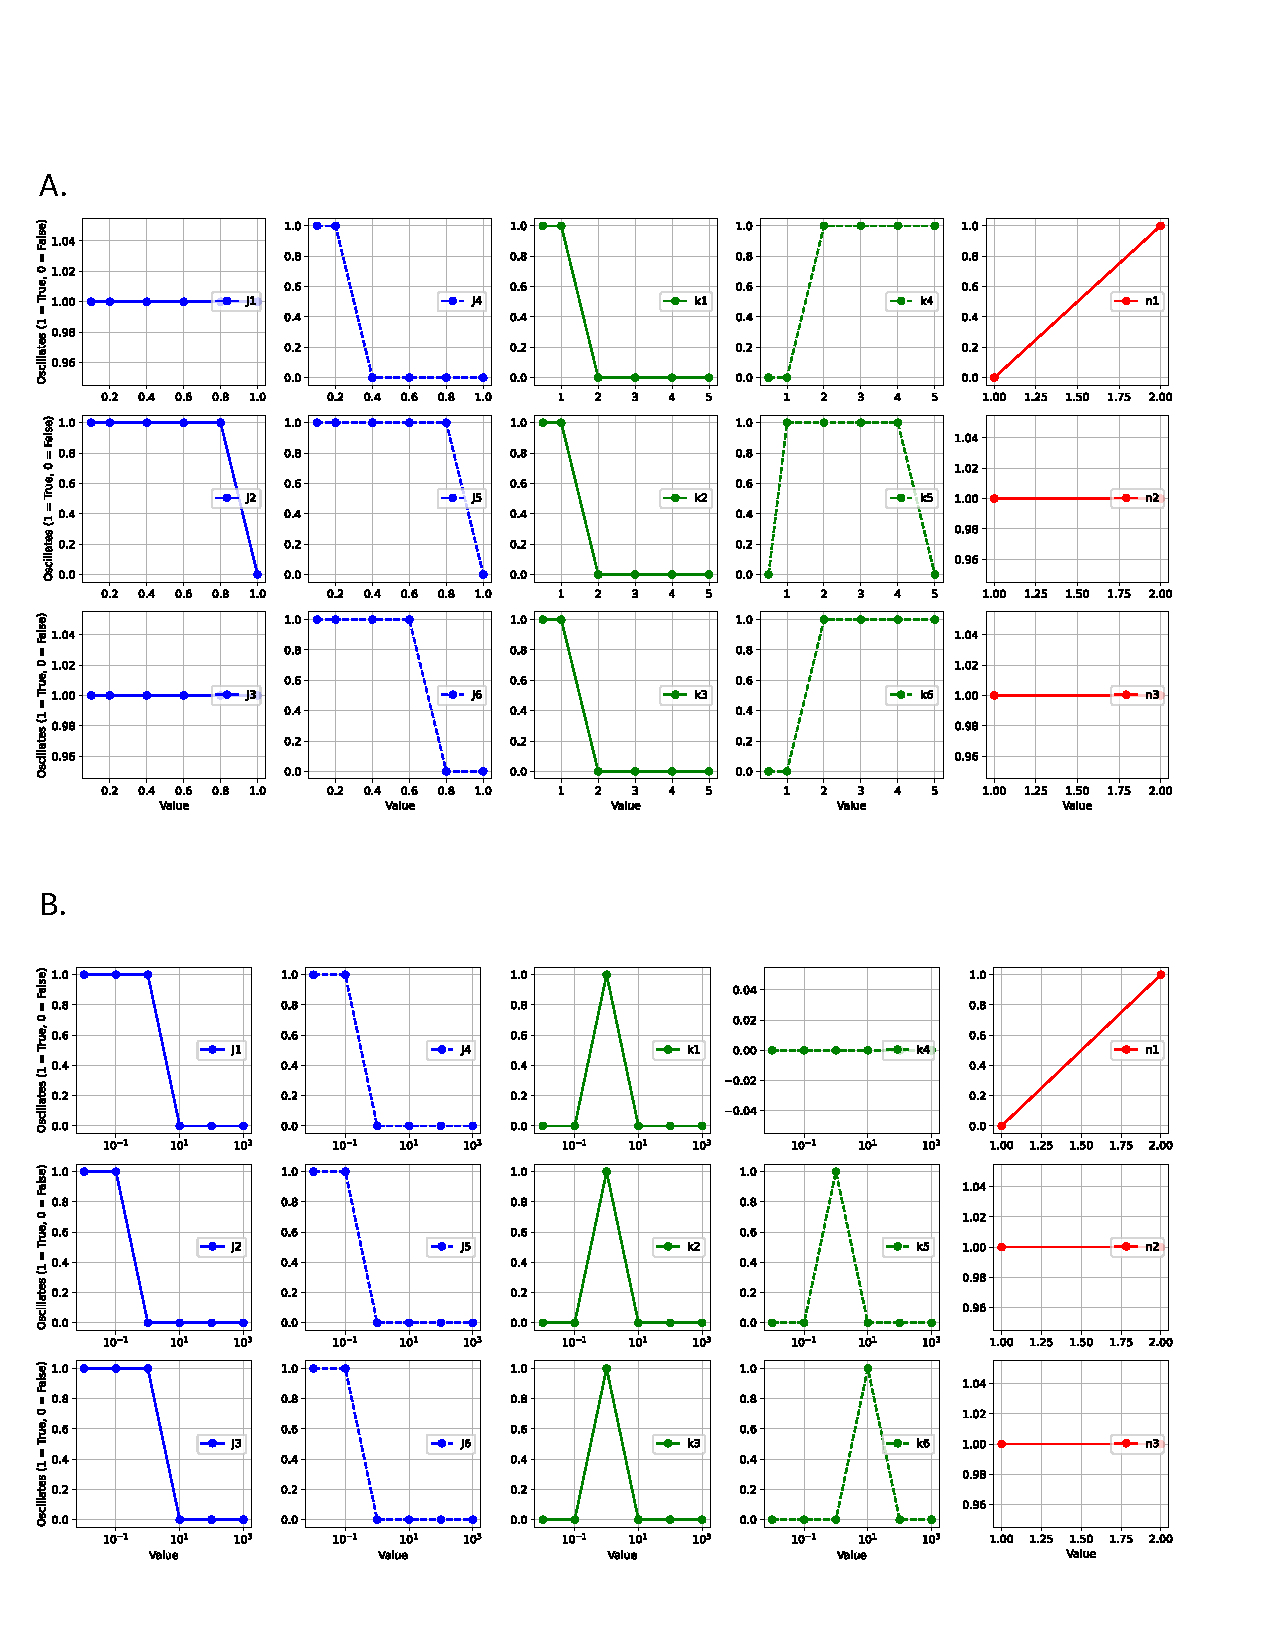
\includegraphics[width=0.7\textwidth]{figure8.pdf}
    \caption{Parameter sweep results for a Represillator + Positive Feedback at \textit{A} model. When the y-value is 1, the concentrations of all three proteins oscillate. When the y-value is 0, the concentration of at least one protein does not oscillate. A. The results of a parameter sweep done using \textit{J} values from 0.1 to 1 and \textit{k} values from 1 to 5. B. The results of a parameter sweep done using \textit{J} and \textit{k} values from \( 10^{-2} \) to \( 10^{2} \) }
    \label{fig:8}
\end{figure}

The results of these parameter sweeps are summarized and compared to previous parameter sweeps in the tables below. As in previous sections, we used \textit{J} values from \( 10^{-2} \) to \( 10^{2} \), \textit{k} values from \( 10^{-2} \) to \( 10^{2} \), and \textit{n} values of 1 and 2.

\begin{table}[H]
\centering
\begin{tabular}{|l|l|l|}
\hline
\textbf{Parameter} & \textbf{Represillator} & \textbf{A} \\
\hline
J1 & 0.1, 0.2, 0.4, 0.6, 0.8, 1 & 0.1, 0.2, 0.4, 0.6, 0.8, 1 \\
J2 & 0.1, 0.2, 0.4, 0.6 & 0.1, 0.2, 0.4, 0.6, 0.8 \\
J3 & 0.1, 0.2, 0.4, 0.6, 0.8, 1 & 0.1, 0.2, 0.4, 0.6, 0.8, 1 \\
J4 & 0.1, 0.2 & 0.1, 0.2 \\
J5 & 0.1, 0.2, 0.4, 0.6, 0.8 & 0.1, 0.2, 0.4, 0.6, 0.8 \\
J6 & 0.1, 0.2, 0.4, 0.6 & 0.1, 0.2, 0.4, 0.6, 0.8 \\
k1 & 0.5, 1 & 0.5, 1 \\
k2 & 0.5, 1 & 0.5, 1 \\
k3 & 0.5, 1 & 0.5, 1 \\
k4 & 2, 3, 4, 5 & 2, 3, 4, 5 \\
k5 & 1, 2, 3, 4 & 1, 2, 3, 4 \\
k6 & 2, 3, 4, 5 & 2, 3, 4, 5 \\
n1 & 2 & 2 \\
n2 & 1, 2 & 1, 2 \\
n3 & 1, 2 & 1, 2 \\
\hline
\end{tabular}
\caption{Parameter Sweep Results on a Small Scale for Represillator and Represillator + Positive Feedback at \textit{A}.}
\end{table}




\begin{table}[H]
\centering
\begin{tabular}{|l|l|l|}
\hline
\textbf{Parameter} & \textbf{Represillator} & \textbf{A} \\
\hline
J1 & 0.01, 0.1, 1 & 0.01, 0.1, 1 \\
J2 & 0.01, 0.1 & 0.01, 0.1 \\
J3 & 0.01, 0.1, 1 & 0.01, 0.1, 1 \\
J4 & 0.01, 0.1 & 0.01, 0.1 \\
J5 & 0.01, 0.1 & 0.01, 0.1 \\
J6 & 0.01, 0.1 & 0.01, 0.1 \\
k1 & 1 & 1 \\
k2 & 1 & 1 \\
k3 & 1 & 1 \\
k4 & None & None \\
k5 & 10 & 1 \\
k6 & 10 & 10 \\
n1 & 2 & 2 \\
n2 & 1, 2 & 1, 2 \\
n3 & 1, 2 & 1, 2 \\
\hline
\end{tabular}
\caption{Parameter Sweep Results on a Log Scale for Represillator and Represillator + Positive Feedback at \textit{A}.}
\end{table}


The addition of a positive feedback does slightly improve robustness to changes in specific parameter values, though it is only seen on a small scale and for specific parameter values (we see no change on the log scale parameter sweep for the \textit{k} and \textit{J} parameters but we see slight changes for the small range sweep). We expected to see a larger improvement in robustness, however the lack of improvement can be explained by the rest of the system being stronger than the effect of \textit{A} activating itself (because when it activates itself, it will then be available to repress more \textit{B}, which will repress more \textit{C}, which then represses more \textit{A}). Building on these results, we added a second positive feedback loop at \textit{B} with the hope that it would offset some of the effect of adding a feedback loop at \textit{A} and improve robustness of the system.  

\subsection{Represillator + Positive Feedback at \textit{A} + \textit{B}}

Using our oscillatory parameters from the previous section and the set of equations previously presented for our new model, we found that the system of a represillator with a positive feedback loop at \textit{A} and \textit{B} does oscillate under the oscillatory parameters for all three proteins as shown in Figure 9. 

%concentration_over_time_A_B_positive_new_equations.pdf 
\begin{figure}[H]
    \centering
    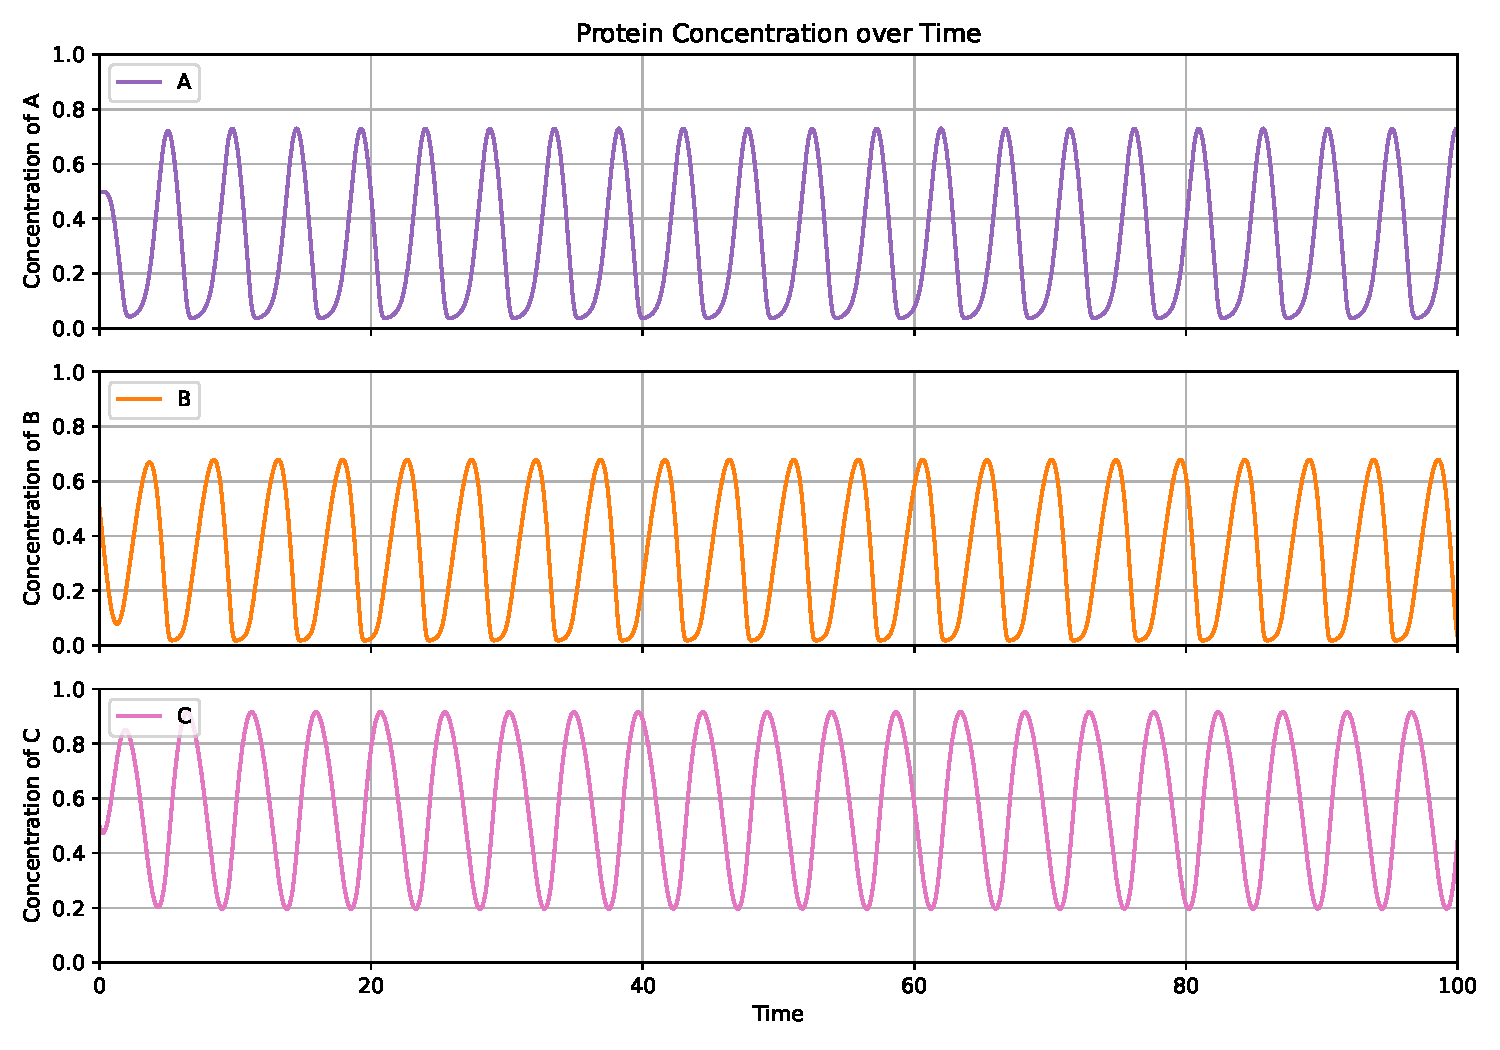
\includegraphics[width=0.7\textwidth]{/Users/olivia/Documents/Fall 2024/MCB 580/MCB580_Challenge3/plots/concentration_over_time_A_B_positive_new_equations.pdf}
    \caption{The behavior of the Represillator + Positive Feedback at \textit{A} + \textit{B} model under oscillatory parameters.}
    \label{fig:9}
\end{figure}



Once we saw that this model was also oscillatory under our parameter set, we tested the robustness of this model compared to the represillator network and network with positive feedback at \textit{A}. Again, using our oscillatory parameters set, we perturbed individual parameters holding the rest constant and examined the range under which the circuit still displayed oscillatory behavior. In Figure 10, the results of our parameter sweep are shown, using the same parameter sweep ranges as the previous section (\textit{J} values from \( 10^{-2} \) to \( 10^{2} \), \textit{k} values from \( 10^{-2} \) to \( 10^{2} \), and \textit{n} values of 1 and 2). 

%oscillatory_behavior_A_B_positive_log_new_equations.pdf, oscillatory_behavior_A_B_positive_new_equations.pdf

\begin{figure}[H]
    \centering
    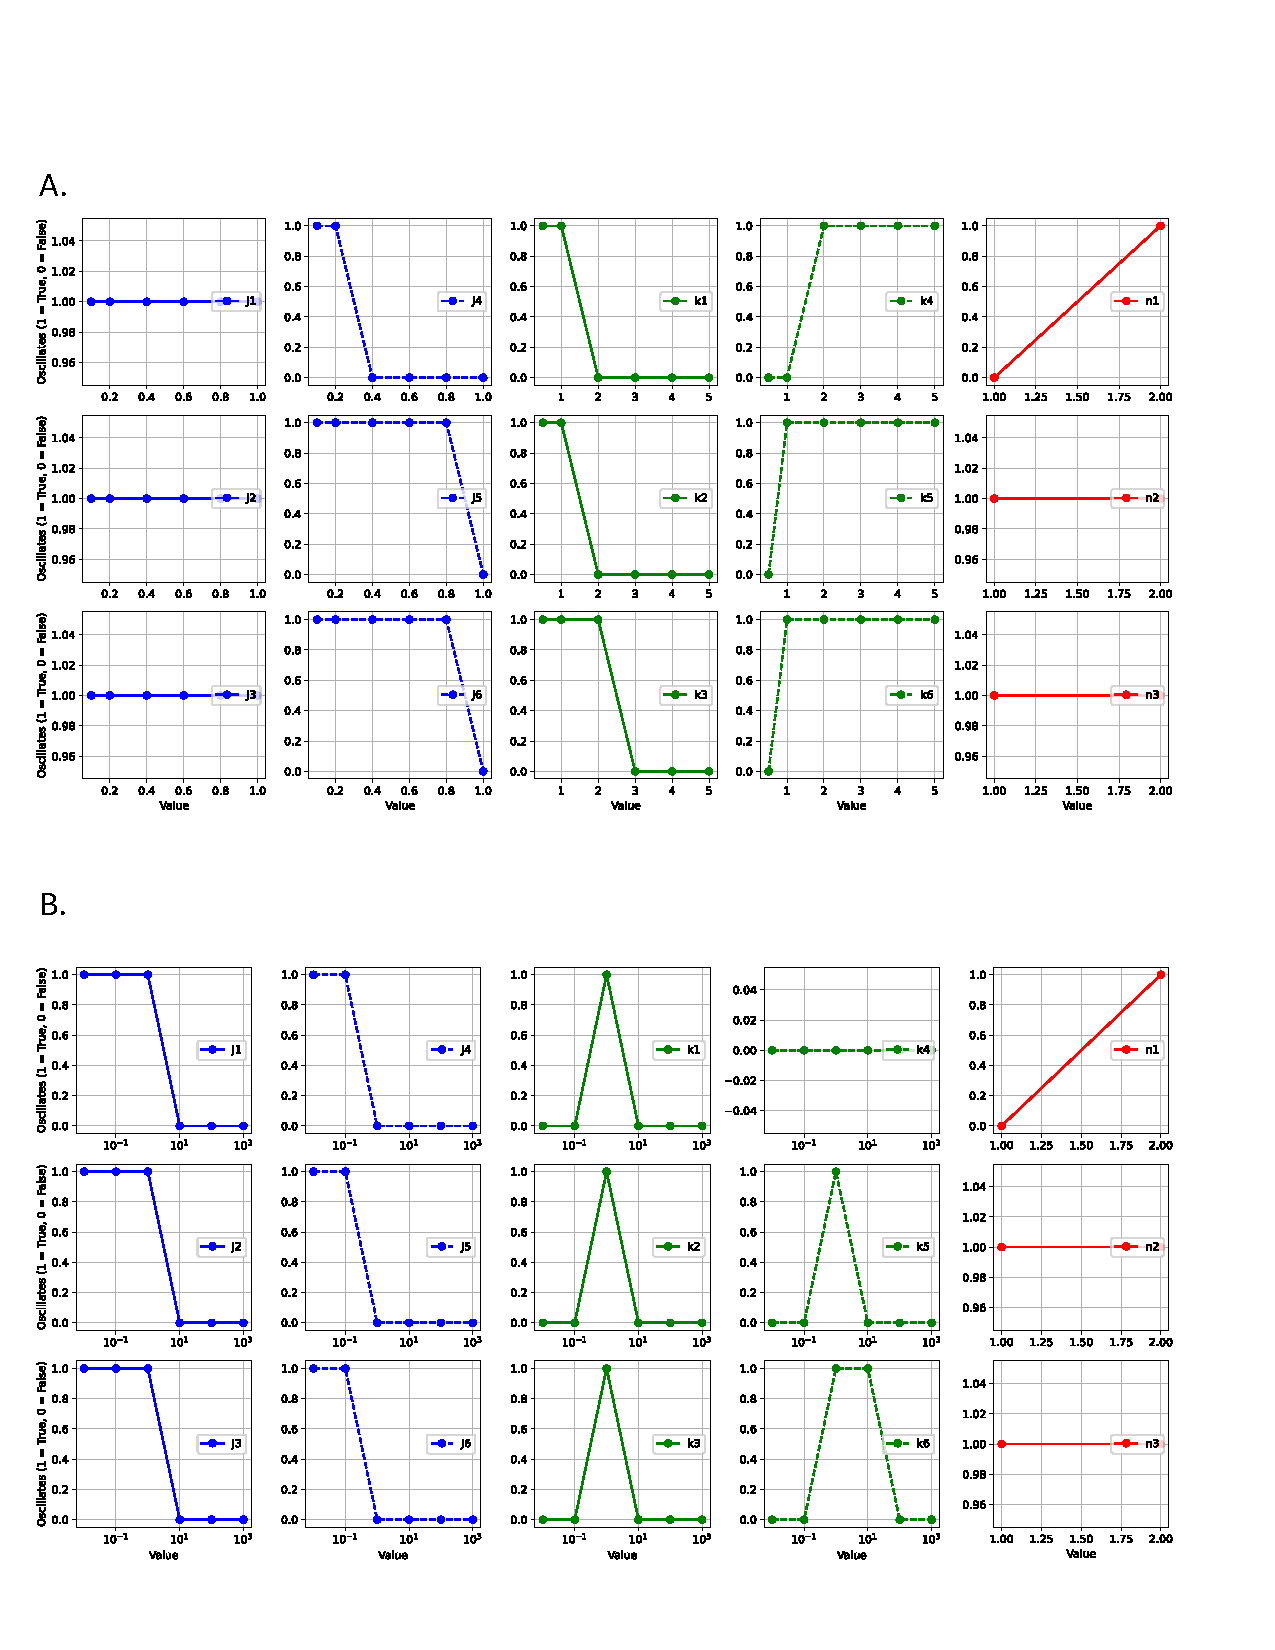
\includegraphics[width=0.7\textwidth]{figure10.pdf}
    \caption{Parameter sweep results for a Represillator + Positive Feedback at \textit{A} + \textit{B} model. When the y-value is 1, the concentrations of all three proteins oscillate. When the y-value is 0, the concentration of at least one protein does not oscillate. A. The results of a parameter sweep done using \textit{J} values from 0.1 to 1 and \textit{k} values from 1 to 5. B. The results of a parameter sweep done using \textit{J} values from \( 10^{-2} \) to \( 10^{2} \), \textit{k} values from \( 10^{-2} \) to \( 10^{2} \). }
    \label{fig:10}
\end{figure}

The results of these parameter sweeps are summarized and compared to previous parameter sweeps in the tables below. As in previous sections, we used \textit{J} values from \( 10^{-2} \) to \( 10^{2} \), \textit{k} values from \( 10^{-2} \) to \( 10^{2} \), and \textit{n} values of 1 and 2.

\begin{table}[H]
\centering
\begin{tabular}{|l|l|l|l|}
\hline
\textbf{Parameter} & \textbf{Represillator} & \textbf{A} & \textbf{A + B} \\
\hline
J1 & 0.1, 0.2, 0.4, 0.6, 0.8, 1 & 0.1, 0.2, 0.4, 0.6, 0.8, 1 & 0.1, 0.2, 0.4, 0.6, 0.8, 1 \\
J2 & 0.1, 0.2, 0.4, 0.6 & 0.1, 0.2, 0.4, 0.6, 0.8 & 0.1, 0.2, 0.4, 0.6, 0.8, 1 \\
J3 & 0.1, 0.2, 0.4, 0.6, 0.8, 1 & 0.1, 0.2, 0.4, 0.6, 0.8, 1 & 0.1, 0.2, 0.4, 0.6, 0.8, 1 \\
J4 & 0.1, 0.2 & 0.1, 0.2 & 0.1, 0.2 \\
J5 & 0.1, 0.2, 0.4, 0.6, 0.8 & 0.1, 0.2, 0.4, 0.6, 0.8 & 0.1, 0.2, 0.4, 0.6, 0.8 \\
J6 & 0.1, 0.2, 0.4, 0.6 & 0.1, 0.2, 0.4, 0.6, 0.8 & 0.1, 0.2, 0.4, 0.6, 0.8 \\
k1 & 0.5, 1 & 0.5, 1 & 0.5, 1 \\
k2 & 0.5, 1 & 0.5, 1 & 0.5, 1 \\
k3 & 0.5, 1 & 0.5, 1 & 0.5, 1, 2 \\
k4 & 2, 3, 4, 5 & 2, 3, 4, 5 & 2, 3, 4, 5 \\
k5 & 1, 2, 3, 4 & 1, 2, 3, 4 & 1, 2, 3, 4, 5 \\
k6 & 2, 3, 4, 5 & 2, 3, 4, 5 & 1, 2, 3, 4, 5 \\
n1 & 2 & 2 & 2 \\
n2 & 1, 2 & 1, 2 & 1, 2 \\
n3 & 1, 2 & 1, 2 & 1, 2 \\
\hline
\end{tabular}
\caption{Parameter Sweep Results on a Small Scale for Represillator, Represillator + Positive Feedback at \textit{A}, and Represillator + Positive Feedback at \textit{A} + \textit{B}.}
\end{table}


\begin{table}[H]
\centering
\begin{tabular}{|l|l|l|l|}
\hline
\textbf{Parameter} & \textbf{Represillator} & \textbf{A} & \textbf{A + B} \\
\hline
J1 & 0.01, 0.1, 1 & 0.01, 0.1, 1 & 0.01, 0.1, 1 \\
J2 & 0.01, 0.1 & 0.01, 0.1 & 0.01, 0.1, 1 \\
J3 & 0.01, 0.1, 1 & 0.01, 0.1, 1 & 0.01, 0.1, 1 \\
J4 & 0.01, 0.1 & 0.01, 0.1 & 0.01, 0.1 \\
J5 & 0.01, 0.1 & 0.01, 0.1 & 0.01, 0.1 \\
J6 & 0.01, 0.1 & 0.01, 0.1 & 0.01, 0.1 \\
k1 & 1 & 1 & 1 \\
k2 & 1 & 1 & 1 \\
k3 & 1 & 1 & 1 \\
k4 & None & None & None \\
k5 & 10 & 1 & 1 \\
k6 & 10 & 10 & 1, 10 \\
n1 & 2 & 2 & 2 \\
n2 & 1, 2 & 1, 2 & 1, 2 \\
n3 & 1, 2 & 1, 2 & 1, 2 \\
\hline
\end{tabular}
\caption{Parameter Sweep Results on a Log Scale for Represillator, Represillator + Positive Feedback at \textit{A}, and Represillator + Positive Feedback at \textit{A} + \textit{B}.}
\end{table}


The addition of a positive feedback does slightly improve robustness to changes in specific parameter values significantly enough that it can be seen on a log scale parameter sweep for \textit{J2}, and \textit{k6} and on a smaller scale parameter sweep for \textit{k2}. The improved robustness to changes in \textit{J2} is likely explained by \textit{B} auto-activating itself, making it less reliant on the repression of \textit{A} by \textit{C} for activation. A similar explanation can be applied to \textit{k2}, with a reduced range compared to \textit{J2} explained by large and small rates being too detrimental to the circuit as a whole. Building on these results, we added one more positive feedback loop at \textit{C}, and tested robustness again.  

\subsection{Represillator + Positive Feedback at \textit{A} + \textit{B} + \textit{C}}

Using our oscillatory parameters from the previous section and the set of equations previously presented for our new model, we found that the system of a represillator with a positive feedback loop at \textit{A} and \textit{B} and \textit{C} does oscillate under the oscillatory parameters for all three proteins as shown in Figure 11. 

%concentration_over_time_A_B_C_positive_new_equations.pdf 
\begin{figure}[H]
    \centering
    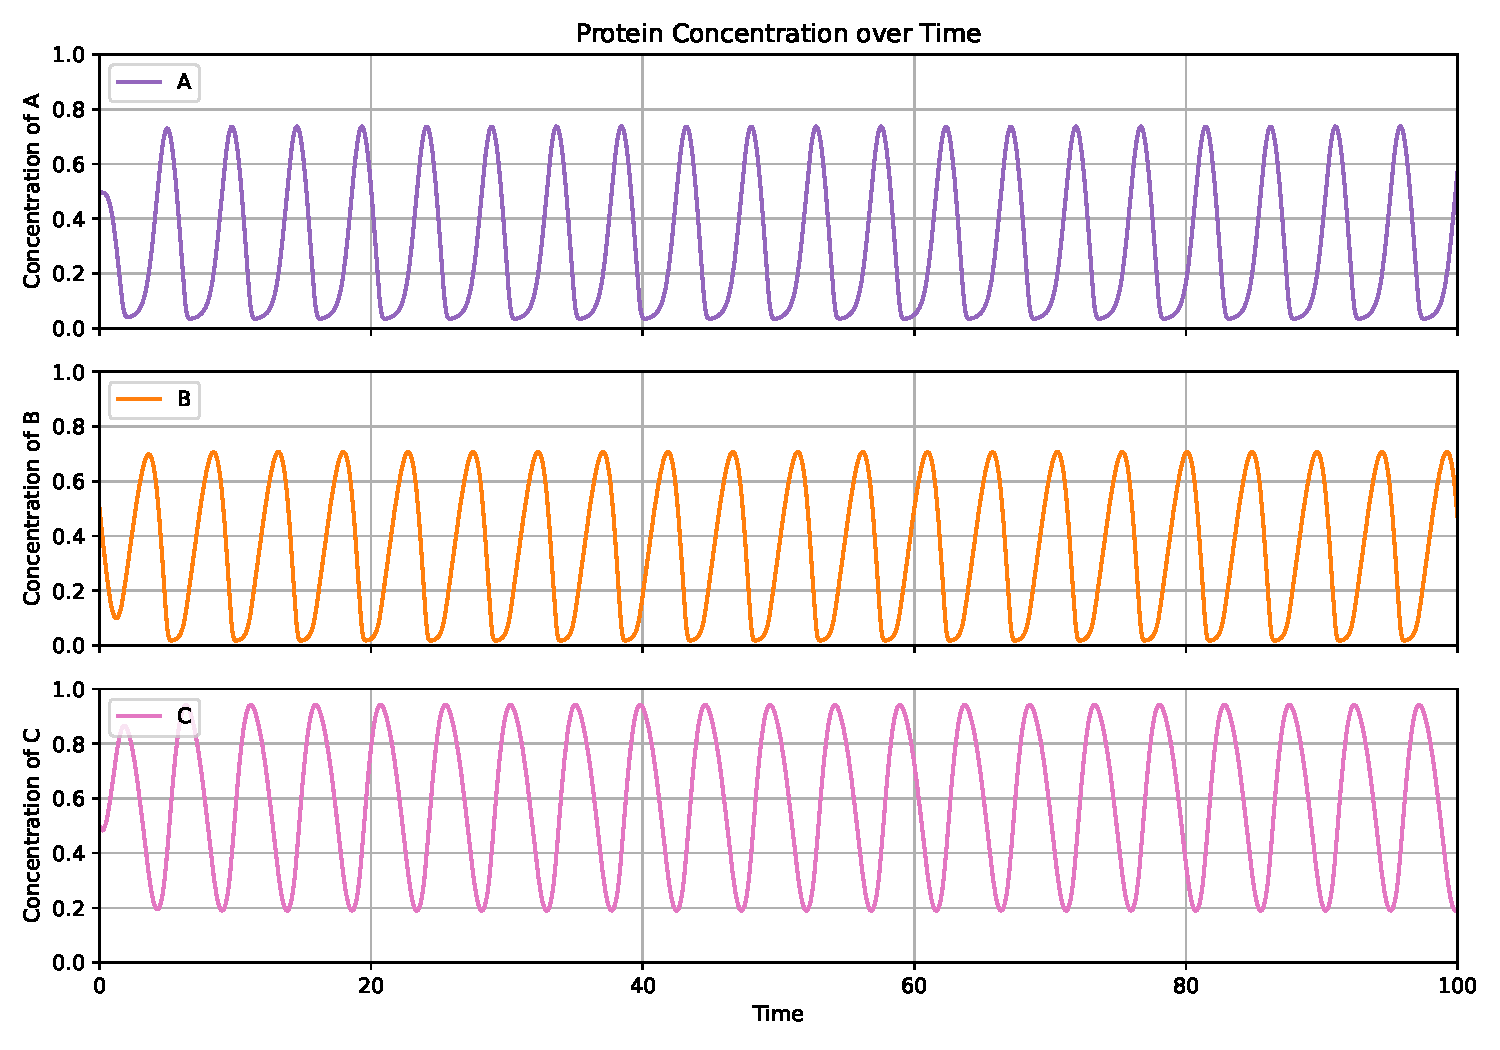
\includegraphics[width=0.7\textwidth]{/Users/olivia/Documents/Fall 2024/MCB 580/MCB580_Challenge3/plots/concentration_over_time_A_B_C_positive_new_equations.pdf}
    \caption{The behavior of the Represillator + Positive Feedback at \textit{A} + \textit{B} + \textit{C} model under oscillatory parameters.}
    \label{fig:11}
\end{figure}



Once we saw that this model was also oscillatory under our parameter set, we tested the robustness of this model compared to the represillator network, network with positive feedback at \textit{A}, and network with positive feedback at \textit{A} and \textit{B}. Again, using our oscillatory parameters set, we perturbed individual parameters holding the rest constant and examined the range under which the circuit still displayed oscillatory behavior. In Figure 12, the results of our parameter sweep are shown, using the same parameter sweep ranges as the previous section (\textit{J} values from \( 10^{-2} \) to \( 10^{2} \), \textit{k} values from \( 10^{-2} \) to \( 10^{2} \), and \textit{n} values of 1 and 2). 

%oscillatory_behavior_A_B_C_positive_log_new_equations.pdf, oscillatory_behavior_A_B_C_positive_new_equations.pdf

\begin{figure}[H]
    \centering
    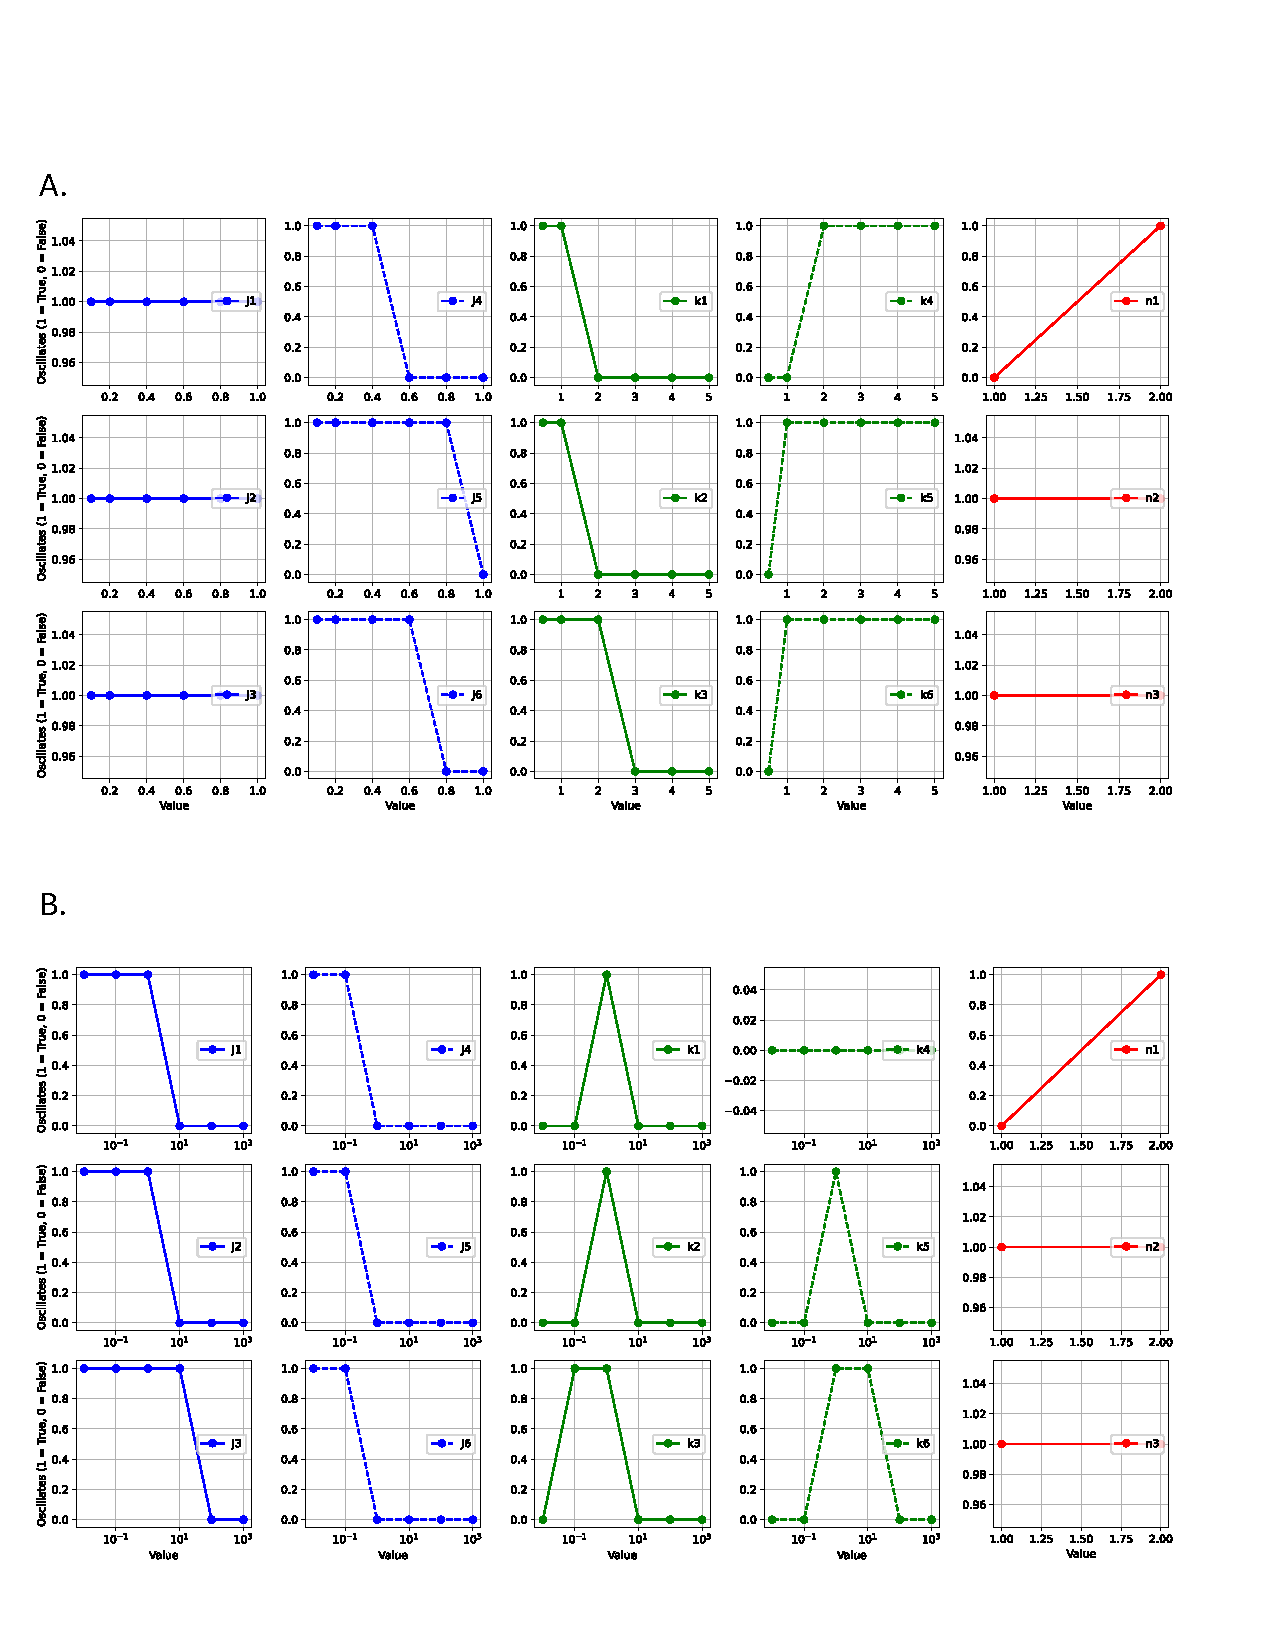
\includegraphics[width=0.7\textwidth]{figure12.pdf}
    \caption{Parameter sweep results for the Represillator + Positive Feedback at \textit{A} + \textit{B} + \textit{C} model. When the y-value is 1, the concentrations of all three proteins oscillate. When the y-value is 0, the concentration of at least one protein does not oscillate. A. The results of a parameter sweep done using \textit{J} values from 0.1 to 1 and \textit{k} values from 1 to 5. B. The results of a parameter sweep done using \textit{J} values from \( 10^{-2} \) to \( 10^{2} \), \textit{k} values from \( 10^{-2} \) to \( 10^{2} \). }
    \label{fig:12}
\end{figure}

The results of these parameter sweeps are summarized and compared to previous parameter sweeps in the tables below. As in previous sections, we used \textit{J} values from \( 10^{-2} \) to \( 10^{2} \), \textit{k} values from \( 10^{-2} \) to \( 10^{2} \), and \textit{n} values of 1 and 2.

\begin{table}[H]
\centering
\begin{tabular}{|l|l|l|l|l|}
\hline
\textbf{Parameter} & \textbf{Represillator} & \textbf{A} & \textbf{A + B} & \textbf{A + B + C}\\
\hline
J1 & 0.1, 0.2, 0.4, 0.6, 0.8, 1 & 0.1, 0.2, 0.4, 0.6, 0.8, 1 & 0.1, 0.2, 0.4, 0.6, 0.8, 1 & 0.1, 0.2, 0.4, 0.6, 0.8, 1 \\
J2 & 0.1, 0.2, 0.4, 0.6 & 0.1, 0.2, 0.4, 0.6, 0.8 & 0.1, 0.2, 0.4, 0.6, 0.8, 1 & 0.1, 0.2, 0.4, 0.6, 0.8, 1 \\
J3 & 0.1, 0.2, 0.4, 0.6, 0.8, 1 & 0.1, 0.2, 0.4, 0.6, 0.8, 1 & 0.1, 0.2, 0.4, 0.6, 0.8, 1 & 0.1, 0.2, 0.4, 0.6, 0.8, 1 \\
J4 & 0.1, 0.2 & 0.1, 0.2 & 0.1, 0.2 & 0.1, 0.2, 0.4 \\
J5 & 0.1, 0.2, 0.4, 0.6, 0.8 & 0.1, 0.2, 0.4, 0.6, 0.8 & 0.1, 0.2, 0.4, 0.6, 0.8 & 0.1, 0.2, 0.4, 0.6, 0.8 \\
J6 & 0.1, 0.2, 0.4, 0.6 & 0.1, 0.2, 0.4, 0.6, 0.8 & 0.1, 0.2, 0.4, 0.6, 0.8 & 0.1, 0.2, 0.4, 0.6 \\
k1 & 0.5, 1 & 0.5, 1 & 0.5, 1 & 0.5, 1 \\
k2 & 0.5, 1 & 0.5, 1 & 0.5, 1 & 0.5, 1 \\
k3 & 0.5, 1 & 0.5, 1 & 0.5, 1, 2 & 0.5, 1, 2 \\
k4 & 2, 3, 4, 5 & 2, 3, 4, 5 & 2, 3, 4, 5 & 2, 3, 4, 5 \\
k5 & 1, 2, 3, 4 & 1, 2, 3, 4 & 1, 2, 3, 4, 5 & 1, 2, 3, 4, 5 \\
k6 & 2, 3, 4, 5 & 2, 3, 4, 5 & 1, 2, 3, 4, 5 & 1, 2, 3, 4, 5 \\
n1 & 2 & 2 & 2 & 2 \\
n2 & 1, 2 & 1, 2 & 1, 2 & 1, 2 \\
n3 & 1, 2 & 1, 2 & 1, 2 & 1, 2 \\
\hline
\end{tabular}
\caption{Parameter Ranges}
\end{table}



\begin{table}[H]
\centering
\begin{tabular}{|l|l|l|l|l|}
\hline
\textbf{Parameter} & \textbf{Represillator} & \textbf{A} & \textbf{A + B} & \textbf{A + B + C} \\
\hline
J1 & 0.01, 0.1, 1 & 0.01, 0.1, 1 & 0.01, 0.1, 1 & 0.01, 0.1, 1 \\
J2 & 0.01, 0.1 & 0.01, 0.1 & 0.01, 0.1, 1 & 0.01, 0.1, 1 \\
J3 & 0.01, 0.1, 1 & 0.01, 0.1, 1 & 0.01, 0.1, 1 & 0.01, 0.1, 1, 10 \\
J4 & 0.01, 0.1 & 0.01, 0.1 & 0.01, 0.1 & 0.01, 0.1 \\
J5 & 0.01, 0.1 & 0.01, 0.1 & 0.01, 0.1 & 0.01, 0.1 \\
J6 & 0.01, 0.1 & 0.01, 0.1 & 0.01, 0.1 & 0.01, 0.1 \\
k1 & 1 & 1 & 1 & 1 \\
k2 & 1 & 1 & 1 & 1 \\
k3 & 1 & 1 & 1 & 0.1, 1 \\
k4 & None & None & None & None \\
k5 & 10 & 1 & 1 & 1 \\
k6 & 10 & 10 & 1, 10 & 1, 10 \\
n1 & 2 & 2 & 2 & 2 \\
n2 & 1, 2 & 1, 2 & 1, 2 & 1, 2 \\
n3 & 1, 2 & 1, 2 & 1, 2 & 1, 2 \\
\hline
\end{tabular}
\caption{Parameter Ranges}
\end{table}


Having positive feedback loops at all three nodes in the circuit does significantly improve robustness to changes in \textit{J1}, \textit{J2}, \textit{J3}, \textit{J4}, \textit{k3}, \textit{k5}, and \textit{k6} compared to the model with no positive feedback loops, although the scale of the improvement in robustness varies depending on which parameter you look at. Compared to the models with only one or two positive feedback loops, we see improvement in robustness to changes in \textit{J2}, \textit{J3}, \textit{J4}, \textit{k3} and \textit{k6}. The improvement in robustness to changes in parameter values that comes from having positive feedback loops at all three nodes is intuitive because as you add feedback loops, you are making the node less dependent on double repression for its own activation since it can activate itself. Compared to adding only one or two positive feedback loops, adding three will have the greatest effect because this decreased dependence on double repression is happening at all three nodes. This result shows that to build a robust biological oscillator using a represillator model, you must incorporate balance in your networks such that if one node is to be less dependent on the interactions between nodes, the other nodes should have the same properties. 


\section{Discussion}

In this paper, we have shown that there is a set of "oscillatory parameters" under which the represillator model presented in Elowitz and Leiler 2000 displays oscillatory behavior \cite{represillator}. We then explored adding feedback loops to one, two, and three nodes in the three node network to explore the robustness of the system. We found that with each additional node, we saw slight improvements in robustness and that the greatest improvement came when adding positive feedback to all three nodes. Just adding positive feedback to one node makes that individual node less dependent on the dynamics of the double repression responsible for its activation, which is reflected in the parameters for the node immediately following it. Adding positive feedback loops to two nodes improved robustness a little bit more, but was still limited because the third node was still fully dependent on double repression for its activation. Having positive feedback at all three nodes showed the largest improvement compared to baseline, which makes sense because now all three nodes are dependent two connected mechanisms for activation (double repression and auto-activation) as opposed to just one (double repression).  

To model this system, we made some assumptions that introduce limitations to our results. One limitation is that when modeling our interactions, we assumed activation to be non-cooperative and repression to be cooperative, so changes to one or both of these assumptions could cause different results. When adding positive feedback loops, we did add a Hill coefficient to represent cooperative activation, suggesting that the molecule is doing something to activate itself, perhaps autophosphorylation. Another limitation of our results is that we limited repression to Hill Coefficients of 1 and 2, meaning that only 1 or 2 binding events respectively is responsible for repression. Biologically, this is reasonable but exceptions or exploring a greater range of parameters here could yield different results. Our hypothesis that adding positive feedback loops would make the system more robust held true to a certain extent, though the effect was limited. As previously discussed, adding a positive feedback loop to a single node does not make that node independent of the other two nodes, but it does reduce dependence on the other nodes. However, because the network is circular, the nodes without positive feedback loops are still affected by the addition of a positive feedback loop to another node. This helps explain why we do not see a significant increase in robustness across multiple parameters until we add positive feedback loops to all three nodes, at which point all three nodes are equally dependent on both themselves and the other two nodes in the system. In our model, we use an input signal, \textit{I}, which we set equal to 1. Increasing or decreasing this value will increase or decrease output of the network. However, you can also remove this term completely and see the exact same behavior presented in this paper, which allows you to model a system that oscillates completely indepdendent of the input. The trade off is that if you remove \textit{I}, input, completely, the system will not respond at all to changes in the input signal, so we decided to leave in this term and keep it equal to 1, allowing for further simulations with increased complexity to show response to signal but keeping it constant to compare robustness across circuit designs as opposed to changing response to different inputs. Despite these limitations our results highlight the importance of having nodes in an oscillator be controlled by multiple mechanisms to have a robust design, which is of biological importance.

Common oscillatory pathways in biological systems include the cell cycle, the segmentation clock, the circadian clock, and calcium oscillations in heart muscle cells \cite{oscillationsinfo}. These biological clocks are essential to life and defects can lead to everything from mild disease to death. Understanding how these systems work and what allows them to function in the face of physiological changes is important to understanding how defects in these pathways can be so detrimental and what we can potentially do therapeutically to mitigate the effects of said defects. Here, we have shown that a simple system of three transactional repressors can oscillate and have displayed that adding positive feedback helps the system be more robust to changes in parameter values, showing that one potential way for biological oscillators to be more robust is to have positive feedback built into systems of repressors. 

\begin{thebibliography}{9}

\bibitem{oscillationsimportance}
Rombouts, J., Verplaetse, S., & Lendert Gelens. (2023). The ups and downs of biological oscillators: a comparison of time-delayed negative feedback mechanisms. \textit{Journal of the Royal Society Interface}, 20(203). https://doi.org/10.1098/rsif.2023.0123

\bibitem{represillator}
Elowitz, M. B., & Leibler, S. (2000). A synthetic oscillatory network of transcriptional regulators. \textit{Nature}, 403(6767), 335–338. https://doi.org/10.1038/35002125

\bibitem{oscillationsinfo}
Li, Z., & Yang, Q. (2017). Systems and synthetic biology approaches in understanding biological oscillators. \textit{Quantitative Biology}, 6(1), 1–14. https://doi.org/10.1007/s40484-017-0120-7

‌


\end{thebibliography}

\end{document}